\documentclass[10pt]{beamer}
\usepackage[utf8]{inputenc}
\usepackage{listings}
\usepackage{xcolor}
\usepackage{makecell}

\usepackage{amsmath}
\usepackage{nccmath}
%\usepackage{showframe}
\usepackage{amssymb} 
\usetheme[progressbar=frametitle]{metropolis}
\usepackage{appendixnumberbeamer}
\usepackage{booktabs}
\usepackage[scale=2]{ccicons}
\usepackage{hyperref}
\hypersetup{
    colorlinks=true,
    linkcolor=blue,
    filecolor=magenta,      
    urlcolor=cyan,
}

\usepackage{pgfplots}
\usepgfplotslibrary{dateplot}

\usepackage{xspace}
\newcommand{\themename}{\textbf{\textsc{metropolis}}\xspace}

\title{Ранжування текстових документів}
%\subtitle{Generic algorithms and performance}
% \date{\today}
\date{}
\author{Тарас Шевченко}
\institute{Rails Reactor / Giphy}
% \titlegraphic{\hfill\includegraphics[height=1.5cm]{logo.pdf}}
\lstdefinestyle{cpp}{
  language=C++,
  stepnumber=1,
  numbersep=10pt,
  tabsize=2,
  showspaces=false,
  showstringspaces=false,
  basicstyle=\scriptsize,
  breaklines
}

\begin{document}

\maketitle

%\begin{frame}{Table of contents}
%  \setbeamertemplate{section in toc}[sections numbered]
%  \tableofcontents[hideallsubsections]
%\end{frame}

\begin{frame}{Компанії, які займаються пошуком}
        \begin{center}
            \begin{figure}
            
\includegraphics[height=8cm,natwidth=1024,natheight=768]{images/search_companies.png}
            \end{figure}
        \end{center}
\end{frame}

\begin{frame}{Як ознайомлювати себе із задачею/кодовою базою}
        \begin{center}
            \begin{figure}
            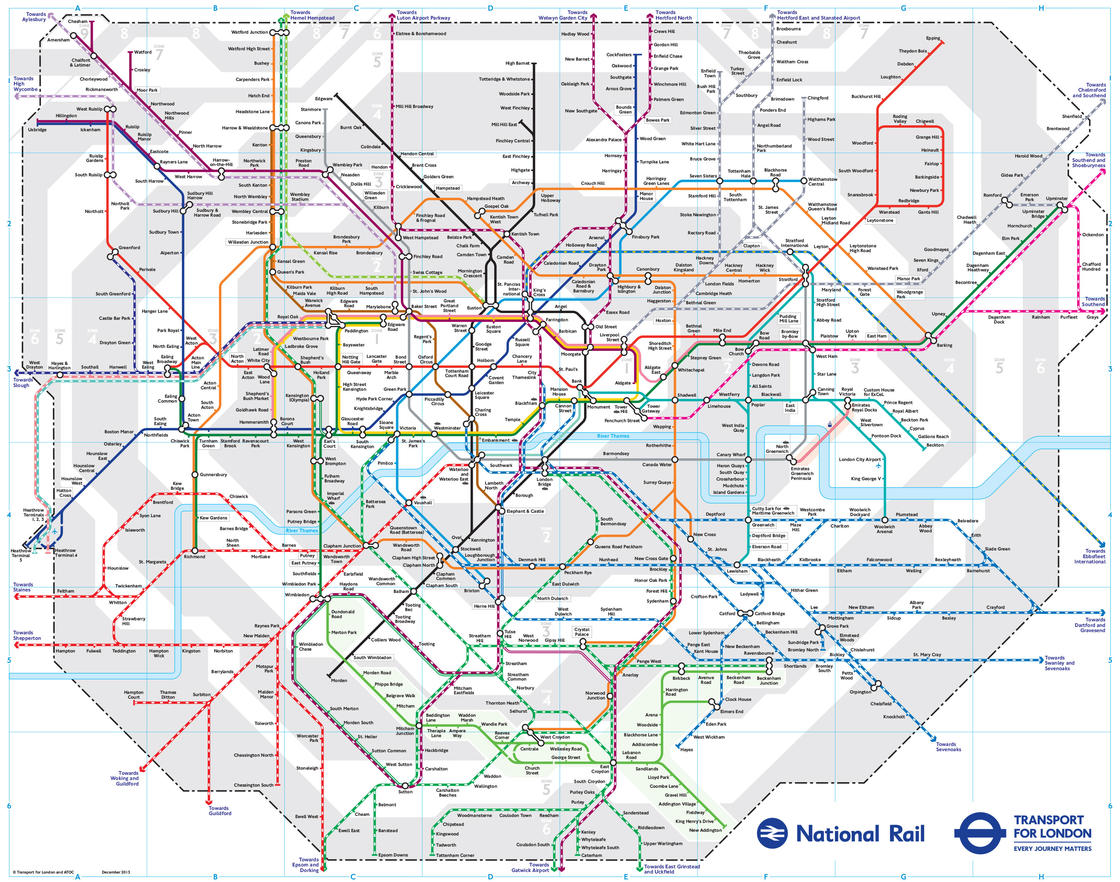
\includegraphics[height=8cm]{images/London_rail.png}
            \end{figure}
        \end{center}
\end{frame}

\begin{frame}{Як ознайомлювати себе із задачею/кодовою базою}
\begin{enumerate}
    \item Пошук у ширину з випадкового місця.
    \item Пошук у глибину з випадкового місця.
    \item Декомпозувати на компоненти та опанувати кожен окремо, а потім зрозуміти як вони зв'язані.
    \item Прослідкувати за формуванням результату.
\end{enumerate}
\end{frame}


\begin{frame}{Ранжування. Спискова видача. Google}
        \begin{center}
            \begin{figure}
            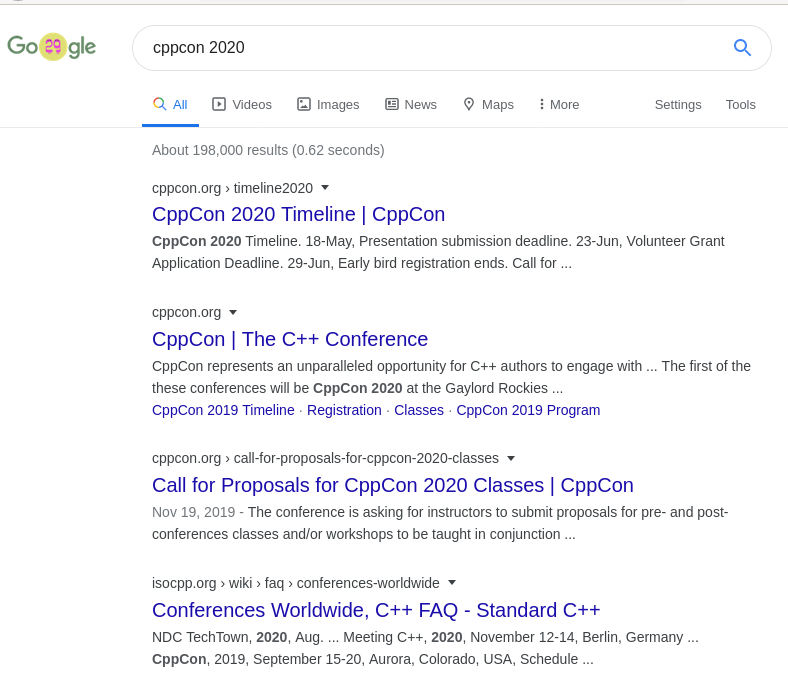
\includegraphics[height=8cm,natwidth=788,natheight=684]{images/search-results.cppcon_2020.google.png}
            \end{figure}
        \end{center}
\end{frame}

\begin{frame}{Ранжування. Спискова видача. Youtube}
        \begin{center}
            \begin{figure}
            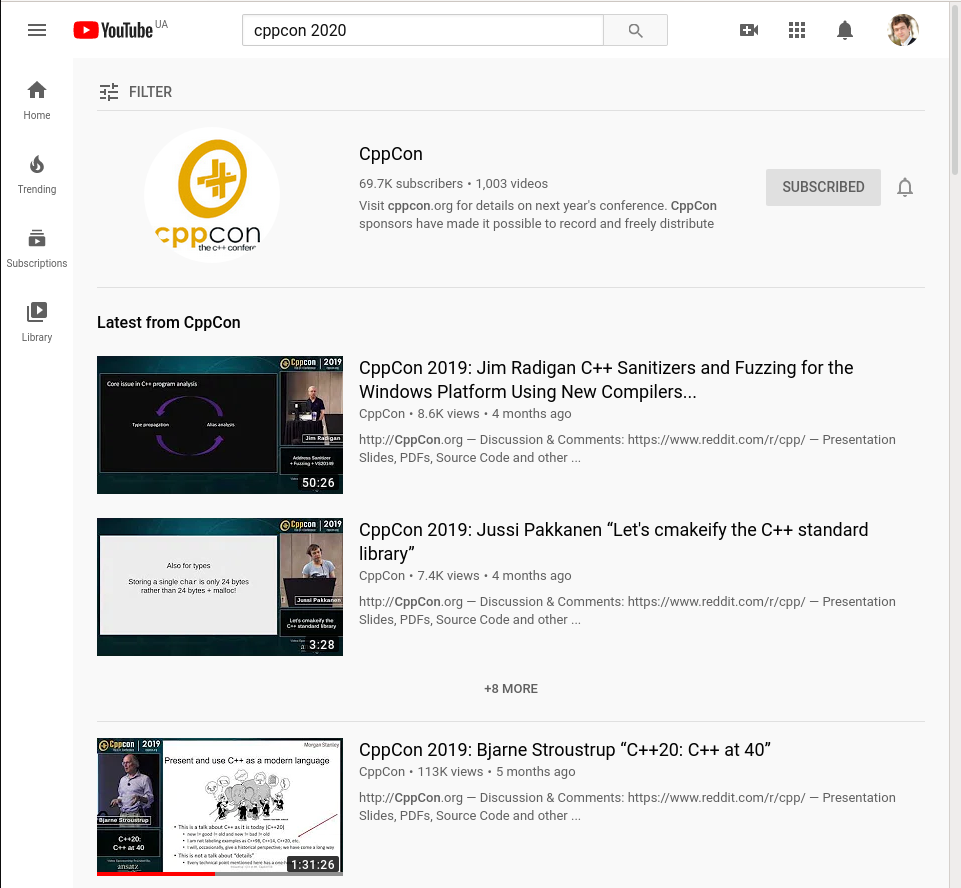
\includegraphics[height=8cm,natwidth=961,natheight=888]{images/search-results.cppcon_2020.youtube.png}
            \end{figure}
        \end{center}
\end{frame}

\begin{frame}{Ранжування. Динамічна сітка. Pinterest}
        \begin{center}
            \begin{figure}
            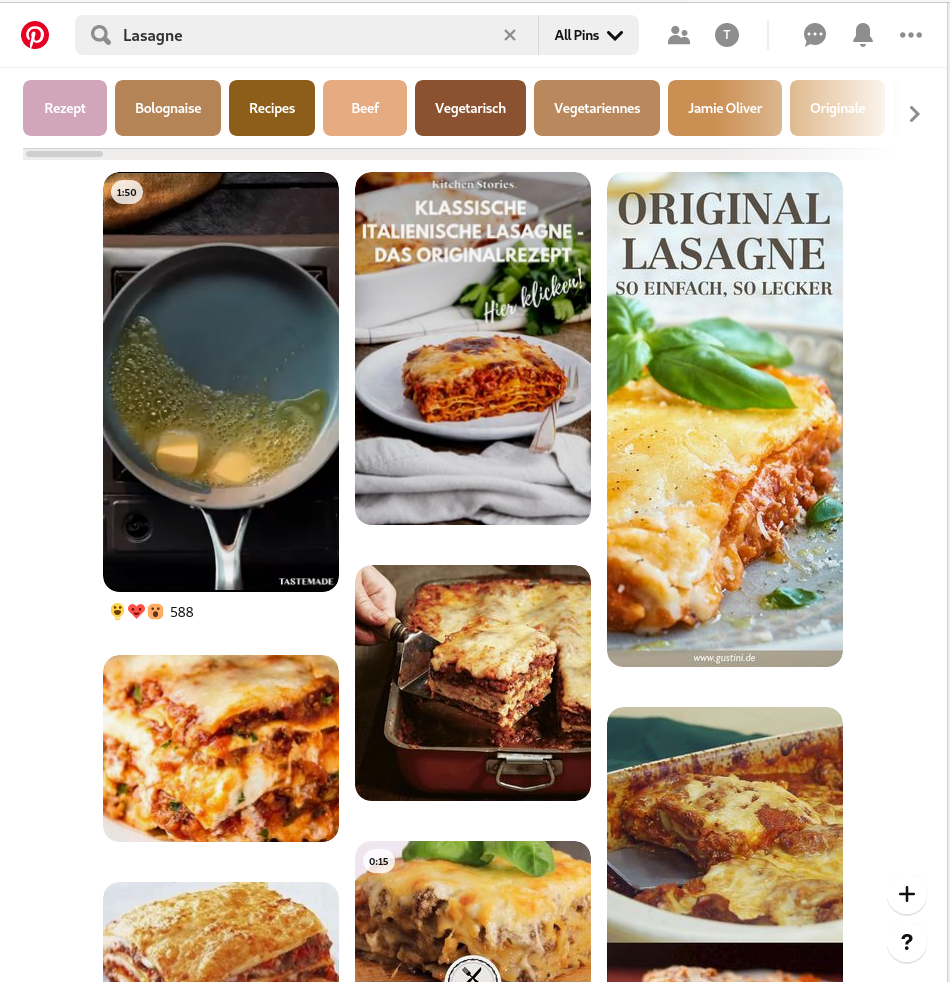
\includegraphics[height=8cm,natwidth=950,natheight=982]{images/search-results.Lasagne.pinterest.png}
            \end{figure}
        \end{center}
\end{frame}

\begin{frame}{Ранжування. Динамічна сітка. Giphy}
        \begin{center}
            \begin{figure}
            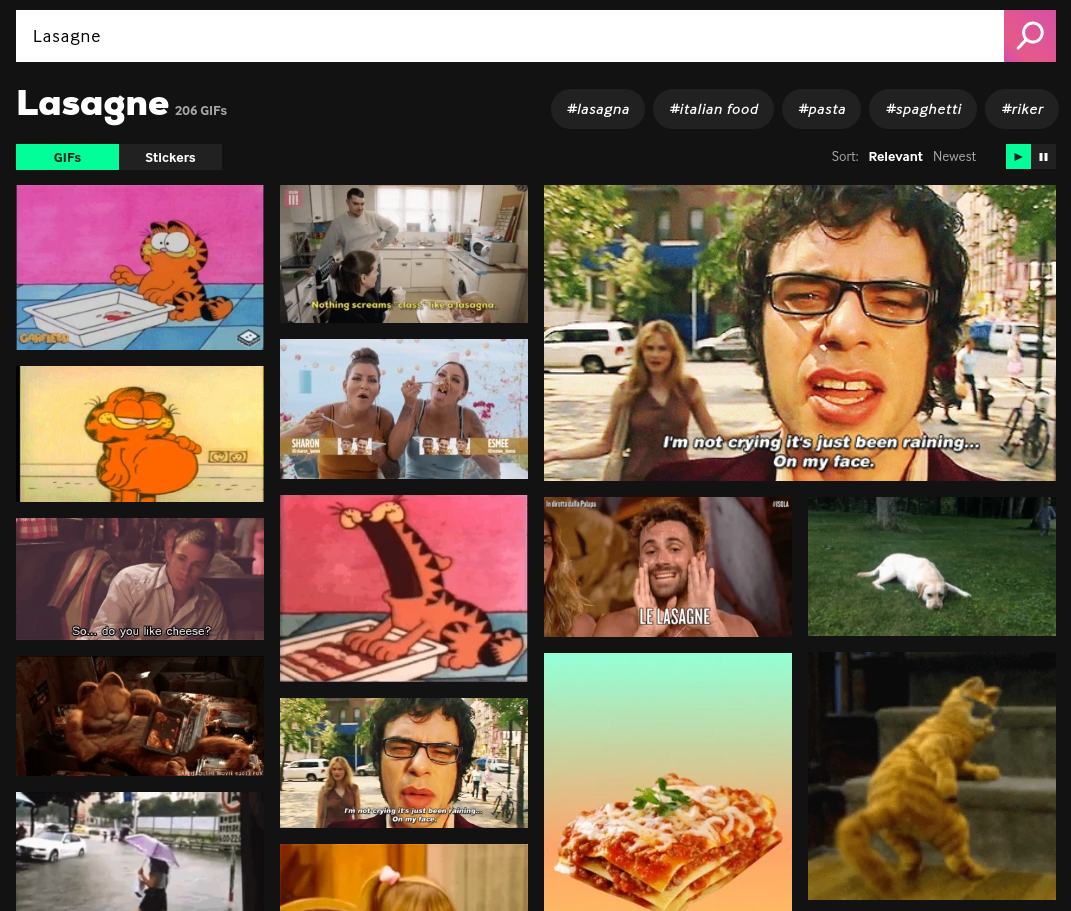
\includegraphics[height=8cm,natwidth=1071,natheight=911]{images/search-results.Lasagne.giphy.png}
            \end{figure}
        \end{center}
\end{frame}

\begin{frame}{Спрощений погляд на пошук}
        \begin{center}
            \begin{figure}
            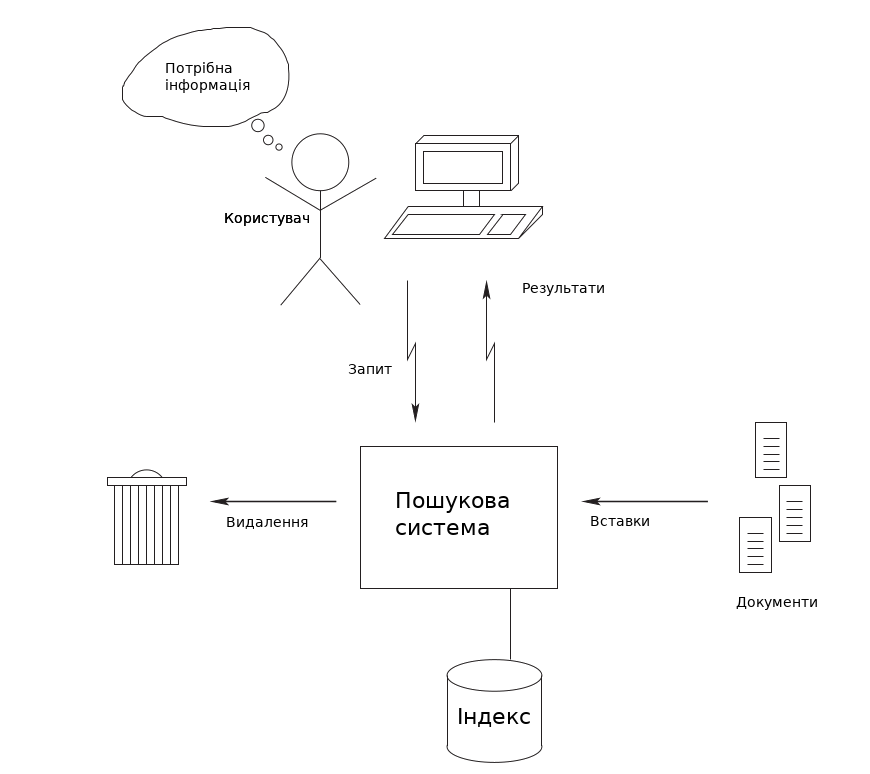
\includegraphics[height=8cm]{images/ir_components_0.png}
            \end{figure}
        \end{center}
\end{frame}

\begin{frame}{Література}
\begin{enumerate}
    \item Christopher D. Manning, Prabhakar Raghavan and Hinrich Schütze, Introduction to Information Retrieval, Cambridge University Press. 2008. 
    \item Christopher Manning, Hinrich Schütze, Foundations of Statistical Natural Language Processing, The MIT Press
    \item  Stefan Büttcher, Charles L. A. Clarke, Gordon V. Cormack, Information Retrieval: Implementing and Evaluating Search Engines, The MIT Press
    \item Hang Li, A Short Introduction to Learning to Rank.
\end{enumerate}
\end{frame}

\begin{frame}{Компоненти системи інформаційного пошуку}
        \begin{center}
            \begin{figure}
            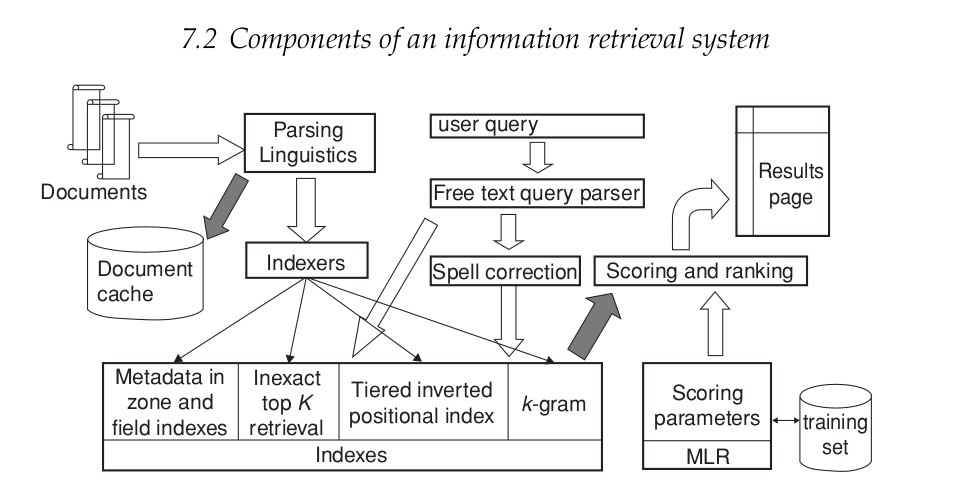
\includegraphics[height=6cm]{images/ir_big_picture.jpg}
            \end{figure}
        \end{center}
\end{frame}


\begin{frame}{Приклад результатів ранжування}
    \begin{center}
    \begin{tabular}{|l|l|}
        \hline
        \thead{Doc ID} & \thead{Score} \\ \hline
        12                   & 153.3 \\ \hline
        23                   & 135.2 \\ \hline
        31                   & 93.12 \\ \hline
        41                   & 80.12 \\ \hline
        54                   & 40.12 \\ \hline
        61                   & 30.12 \\ \hline
        27                   & 25.12 \\ \hline
        38                   & 25.12 \\ \hline
        99                   & 25.12 \\ \hline
    \end{tabular}
    \end{center}
\end{frame}

\begin{frame}{Найпростіша формула ранжування, яка може дати прийнятний результат}
$$BM25(D, Q) = \sum_{i=1}^{n}{\frac{N - n(q_{i}) + 0.5}{n(q_{i}) + 0.5}} * \frac{f(q_{i}, D)(k_{1} + 1)}{f(q_{i}, D) + k_{1}(1 - b + b\frac{|D|}{avgdl})}$$
    \begin{center}
    \begin{tabular}{|l|l|}
        \hline
        \thead{Символ} & \thead{Пояснення} \\ \hline
        $N$ & кількість документів у колекції \\ \hline
        $n$ & кількість слів у запиті \\ \hline
        $q_{i}$ & i-те слово запиту \\ \hline
        $n(q_{i})$& кількість документів, в яких зустрічається слово $q_{i}$. \\ \hline
        $f(q_{i}, D)$& скільки разів зустрічається слово $q{i}$ у документі. \\ \hline
        $|D|$& довжина документу $D$\\ \hline
        $avgdl$& серденя довжина документу\\ \hline
        $k_{i}$& $[1.2, 2.0]$\\ \hline
        $b$& 0.75 \\ \hline
    \end{tabular}
    \end{center}
\end{frame}


\begin{frame}{Недоліки Okapi BM25}
\begin{enumerate}
    \item не враховує позицію в документі;
    \item не праховує особливостей мови
\end{enumerate}
\end{frame}

\begin{frame}{Okapi}
    \begin{figure}
        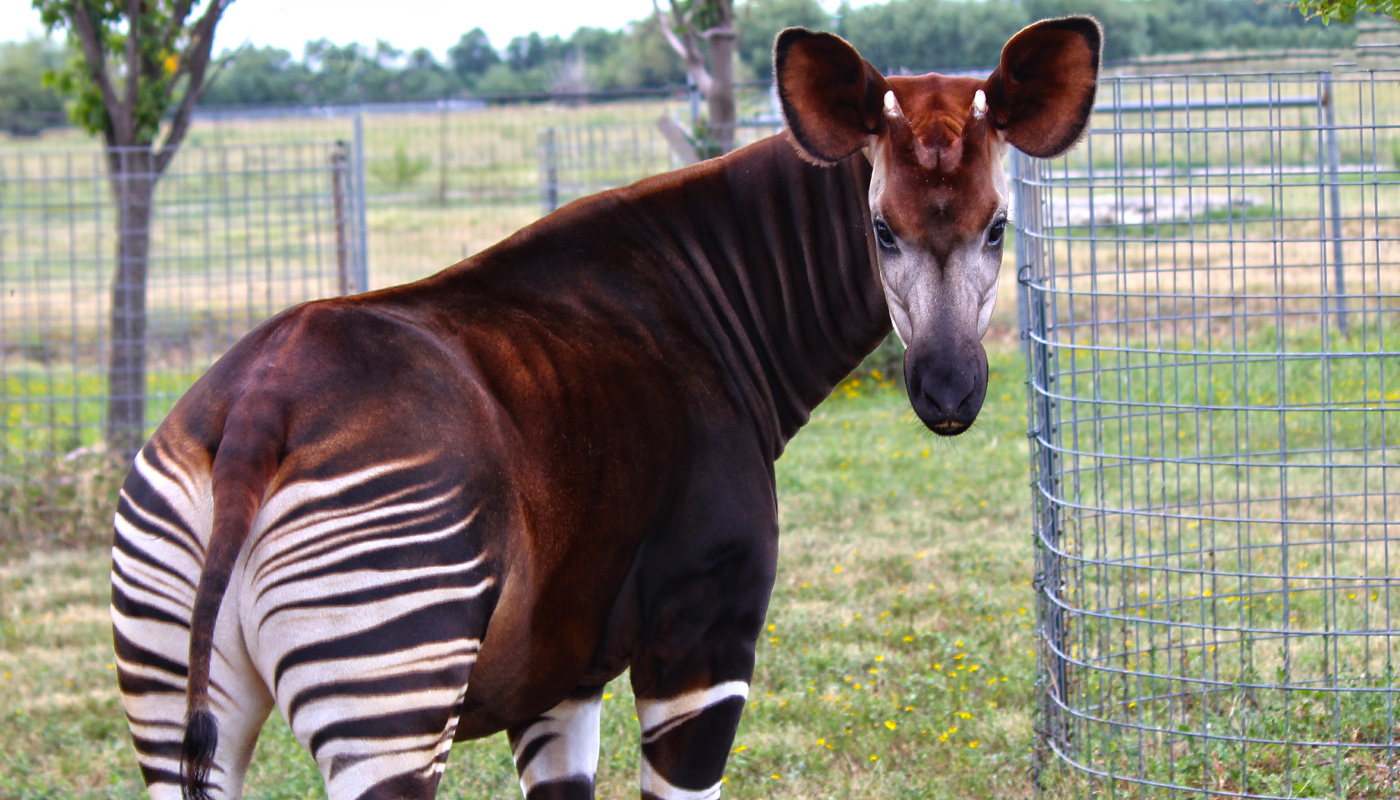
\includegraphics[height=6cm]{images/okapi.jpg}
    \end{figure}
\end{frame}



\begin{frame}{Структура логу записів}
\begin{center}
\begin{tabular}{|l|l|l|}
    \hline
    \thead{Doc ID} & \thead{Score} &\thead{Query} \\ \hline
    12                  & 153.3         & чай \\ \hline
    23                  & 135.2         & чай \\ \hline
    31                  & 93.12         & чай \\ \hline
    41                  & 80.12         & чай \\ \hline
    54                  & 40.12         & чай \\ \hline
    61                  & 30.12         & чай \\ \hline
    27                  & 25.12         & чай \\ \hline
    38                  & 25.12         & чай \\ \hline
    99                  & 25.12         & чай \\ \hline
\end{tabular}
\end{center}
\end{frame}


\begin{frame}{Структура логу записів}
\begin{center}
\begin{tabular}{|l|l|l|l|l|l|l|l|l|l|l|l|}
    \hline
\thead{ts}&   \thead{DID} & \thead{S}  & \thead{Query} & \thead{QL}    & \thead{RID}  & \thead{SID} & \thead{MID}  & \thead{A} & \thead{UID}& \thead{IP}& \thead{CC} \\ \hline
13        &     12          & 95         & чай           & UK             & e1q          & fbde        & 1         & V         & 13         & - & UA \\  \hline
13        &     23          & 94         & чай           & UK             & e1q          & fbde        & 1         & V         & 13         & - & UA \\  \hline
13        &     31          & 93         & чай           & UK             & e1q          & fbde        & 1         & V         & 13         & - & UA \\  \hline
13        &     41          & 80         & чай           & UK             & e1q          & fbde        & 1         & V         & 13         & - & UA \\  \hline
13        &     54          & 40         & чай           & UK             & e1q          & fbde        & 1         & V         & 13         & - & UA \\  \hline
13        &     61          & 30         & чай           & UK             & e1q          & fbde        & 1         & V         & 13         & - & UA \\  \hline
13        &     27          & 25         & чай           & UK             & e1q          & fbde        & 1         & V         & 13         & - & UA \\  \hline
13        &     38          & 24         & чай           & UK             & e1q          & fbde        & 1         & V         & 13         & - & UA \\  \hline
13        &     99          & 23         & чай           & UK             & e1q          & fbde        & 1         & V         & 13         & - & UA \\  \hline
\end{tabular}
\end{center}
\end{frame}


\begin{frame}{Вибір ключу для сортування логу запитів}
\begin{center}
\begin{tabular}{|l|l|}
    \hline
    \thead{Ключ}          & \thead{Переваги} \\ \hline
    <ts, sid, rid>        & Швидкість запису \\ \hline
    <A, ts, sid, rid>     & \makecell[l]{Відсутність необхідності сканувати дані для дій,\\які не беруть участь у запиті.}  \\ \hline
    <A, ql, ts, sid, rid> & \makecell[l]{Дозволяє ефективніше програховувати запити\\різних мов.}   \\ \hline
\end{tabular}
\end{center}
\end{frame}


\begin{frame}{Розмітка даних}
        \begin{center}
            \begin{figure}
            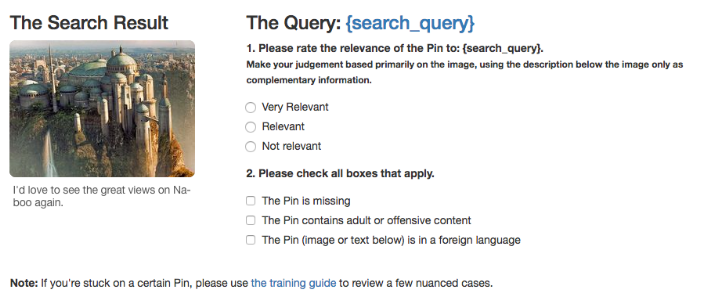
\includegraphics[height=5cm]{images/accessors_job.png}
            \end{figure}
        \end{center}
\end{frame}

\begin{frame}{Поради стосовно розмітки даних}
\begin{enumerate}
    \item випадково обирайте запити для тренувальної вибірки, враховуючи частість запитів;
    \item обирайте документи так, щоб покрити якомога ширший діапазон значень ваших ознак, які будете використовувати;
    \item власноруч розмітьте кілька сотень пар;
    \item обирайте від трьох до 5-ти мір релевантності;
    \item враховуйте специфіку вашої предметної області (можливо, варто внести варіант виду "аксесуар до пристрою, який згадувався у запиті").
    \item застосовуйте статистичні методи оцінки узгодженості результатів
\end{enumerate}
\end{frame}


\begin{frame}{Поради стосовно розмітки даних}
\begin{enumerate}
    \item правильно підбирайте тестові запитання;
    \item слідкуйте за процесом розмітки;
    \item вимагайте як мінімум 3 голоси для оцінки якості пари;
    \item обирайте не менше десяти документів для 1-го запиту.
\end{enumerate}
\end{frame}

\begin{frame}{Оцінка поточного алгоритму сортування}
\begin{columns}
\begin{column}{0.5\textwidth}
\begin{tabular}{|l|l|l|l|l|}
    \hline
    \thead{№} & \thead{Doc ID} & \thead{Query} & \thead{Score} & \thead{Rel}  \\ \hline
    1    &12                  & чай            & 153.3              & 1 \\ \hline
    2    &23                  & чай            & 135.2              & 2 \\ \hline
    3    &31                  & чай            & 93.12              & 3 \\ \hline
    4    &41                  & чай            & 80.12              & 4 \\ \hline
\end{tabular}
\end{column}

\begin{column}{0.5\textwidth}
\begin{tabular}{|l|l|l|l|l|}
    \hline
    \thead{№} & \thead{Doc ID} & \thead{Query} & \thead{Score} & \thead{Rel}  \\ \hline
    1         &    41                  & чай            & 80.12              & 4 \\ \hline
    2         &    31                  & чай            & 93.12              & 3 \\ \hline
    3         &    23                  & чай            & 135.2              & 2 \\ \hline
    4         &    12                  & чай            & 153.3              & 1 \\ \hline
\end{tabular}
\end{column}
\end{columns}
$$MRR = \frac{1}{|Q|} \sum_{i=1}^{|Q|}{\frac{1}{r_{i}}} = \frac{1}{1} * (\frac{1}{3})$$
$$nDCG_{p} = \frac{DCG_{p}}{IDCG_{p}} = \frac{\sum_{i=1}^{p}{\frac{rel_{i}}{log_{2}{(i + 1)}}}}{\sum_{i=1}^{p}{\frac{rel_{x_{i}}}{log_{2}{(i + 1)}}}} = \frac{\frac{1}{log_{2}{2}} + \frac{2}{log_{2}{3}} + \frac{3}{log_{2}{4}}  + \frac{4}{log_{2}{5}}}{\frac{4}{log_{2}{2}} + \frac{3}{log_{2}{3}} + \frac{2}{log_{2}{4}}  + \frac{1}{log_{2}{5}}} \approx \frac{5.48}{7.32} \approx 0.75 $$
\begin{align*}
&PairAccuracy = \frac{1}{|\{(i, j) | rel_{i} \prec rel_{j}\}|}\sum_{\{(i, j) | rel_{i} \prec rel_{j}\}}^{}{[score_{i} \prec score_{j}]} = \\
&=([153.3 < 135.2] +  [153.3 < 93.12] +  [153.3 < 80.12] + \\
&+[135.2 < 93.12] + [135.2 < 80.12] + [93.12 < 80.12]) / 6 = 0.0
\end{align*}
\end{frame}


\end{document}
